%!Mode:: "TeX:UTF-8"
\section{数据库优化}

数据库优化措施包括:
\begin{itemize}
    \item 索引
    \item 拆分
    \item 读写分离
    \item 缓存,如memcached
    \item 优化SQL语句,减少不必要的where,order by, select语句不使用*, 减少访问数据库次数(宁可集中批量操作,避免频繁读写)
\end{itemize}

\subsection{数据库拆分(分布式)}

\begin{itemize}
    \item 垂直(纵向)拆分:是指按功能模块拆分,比如分为订单库、商品库、用户库...这种方式多个数据库之间的表结构不同。
    \item 水平(横向)拆分:将同一个表的数据进行分块保存到不同的数据库中,这些数据库中的表结构完全相同
	\begin{itemize}
    		\item 顺序拆分,如可以按订单的日前按年份才分,2003年的放在db1中,2004年的db2,以此类推。当然也可以按主键标准拆分。
    		\item hash取模分,优点是分布均匀
		\item 增加一层数据库维护拆分映射关系,优点是灵活性强	
	\end{itemize}
\end{itemize}


\subsection{读写分离}
基本的原理是让主数据库处理事务性查询,而从数据库处理SELECT查询。
数据库复制被用来把事务性查询导致的变更同步到集群中的从数据库。
读写分离简单的说是把对数据库读和写的操作分开对应不同的数据库服务器,这样能有效地减轻数据库压力,也能减轻IO压力。
主数据库提供写操作,从数据库提供读操作,其实在很多系统中,主要是读的操作。
当主数据库进行写操作时,数据要同步到从的数据库,这样才能有效保证数据库完整性。

\begin{figure}[ht]
	\begin{center}
		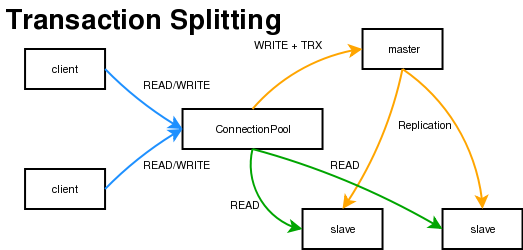
\includegraphics[keepaspectratio,width=0.5\paperwidth]{Pictures/Network/EbayRWSplitting.png}
	\caption{Ebay的读写分离}
	\label{fig:VirtualServer}
	\end{center}
\end{figure}

\begin{figure}[ht]
	\begin{center}
		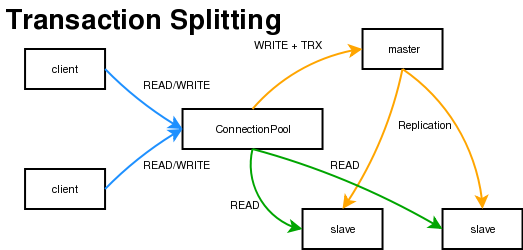
\includegraphics[keepaspectratio,width=0.5\paperwidth]{Pictures/Network/MySQLSplitting.png}
	\caption{MySQL的读写分离}
	\label{fig:VirtualServer}
	\end{center}
\end{figure}


Ebay使用Oracle的数据库,通过Quest SharePlex工具进行数据同步。

MySQL也有自己的同步数据技术, 通过日志在从数据库重复主数据库的操作达到异步复制数据目的。



\subsection{索引}

索引是对数据库表中一列或多列的值进行排序的一种结构,使用索引可快速访问数据库表中的特定信息。
建立索引的目的是加快对表中记录的\textbf{查找}或\textbf{排序}。为表设置索引要付出代价的:一是增加了数据库的存储空间,二是在插入和修改数据时要花费较多的时间(因为索引也要随之变动)。
数据库索引就是为了提高表的搜索效率而对某些字段中的值建立的目录 。

创建索引可以大大提高系统的性能。第一,通过创建唯一性索引,可以保证数据库表中每一行数据的唯一性。第二,可以大大加快数据的检索速度,这也是创建索引的最主要的原因。第三,可以加速表和表之间的连接,特别是在实现数据的参考完整性方面特别有意义。第四,在使用分组和排序子句进行数据检索时,同样可以显著减少查询中分组和排序的时间。第五,通过使用索引,可以在查询的过程中,使用优化隐藏器,提高系统的性能。

例如这样一个查询:select * from table1 where id=10000。如果没有索引,必须遍历整个表,直到ID等于10000的这一行被找到为止;有了索引之后(必须是在ID这一列上建立的索引),即可在索引中查找。由于索引是经过某种算法优化过的,因而查找次数要少的多的多。可见,索引是用来定位的。

索引分为\textbf{聚簇索引}和\textbf{非聚簇索引}两种,聚簇索引是按照数据存放的物理位置为顺序的,而非聚簇索引就不一样了;聚簇索引能提高多行检索的速度,而非聚簇索引对于单行的检索很快。

根据数据库的功能,可以在数据库设计器中创建三种索引:唯一索引、主键索引和聚集索引。


唯一索引是不允许其中任何两行具有相同索引值的索引。
当现有数据中存在重复的键值时,大多数数据库不允许将新创建的唯一索引与表一起保存。数据库还可能防止添加将在表中创建重复键值的新数据。例如,如果在employee表中职员的姓(lname)上创建了唯一索引,则任何两个员工都不能同姓。

在数据库关系图中为表定义主键将自动创建主键索引,主键索引是唯一索引的特定类型。该索引要求主键中的每个值都唯一。当在查询中使用主键索引时,它还允许对数据的快速访问。

在\textbf{聚集索引}中,表中行的物理顺序与键值的逻辑(索引)顺序相同。一个表只能包含一个聚集索引。
如果某索引不是聚集索引,则表中行的物理顺序与键值的逻辑顺序不匹配。与非聚集索引相比,聚集索引通常提供更快的数据访问速度。

\textbf{应该在这些列上创建索引}

\begin{itemize}
    \item 
在经常需要搜索的列上,可以加快搜索的速度
    \item 
在作为主键的列上,强制该列的唯一性和组织表中数据的排列结构
    \item 
在经常用在连接的列上,这些列主要是一些外键,可以加快连接的速度;
    \item 
在经常需要根据范围进行搜索的列上创建索引,因为索引已经排序,其指定的范围是连续的;
    \item 
在经常需要排序的列上创建索引,因为索引已经排序,这样查询可以利用索引的排序,加快排序查询时间;
    \item 
在经常使用在WHERE子句中的列上面创建索引,加快条件的判断速度
\end{itemize}

\textbf{不应该在这些列上创建索引}

\begin{itemize}
    \item 
第一,对于那些在查询中很少使用或者参考的列不应该创建索引。这是因为,既然这些列很少使用到,因此有索引或者无索引,并不能提高查询速度。相反,由于增加了索引,反而降低了系统的维护速度和增大了空间需求。
    \item 
第二,对于那些只有很少数据值的列也不应该增加索引。这是因为,由于这些列的取值很少,例如人事表的性别列,在查询的结果中,结果集的数据行占了表中数据行的很大比例,即需要在表中搜索的数据行的比例很大。增加索引,并不能明显加快检索速度。
    \item 
第三,对于那些定义为text, image和bit数据类型的列不应该增加索引。这是因为,这些列的数据量要么相当大,要么取值很少,不利于使用索引。
    \item 
第四,当修改性能远远大于检索性能时,不应该创建索引。这是因为,修改性能和检索性能是互相矛盾的。当增加索引时,会提高检索性能,但是会降低修改性能。当减少索引时,会提高修改性能,降低检索性能。因此,当修改操作远远多于检索操作时,不应该创建索引。
\end{itemize}

\clearpage













